\section{Introduction}

% Tracing algorithms is ubiquitous, fundamental
Tracing algorithms on concrete examples is fundamental to teaching and learning
in CS education~\cite{Lister2004}. Drawing traces on blackboards and paper is
common practice (\fig{fig:6006-insertion}), 
%%% first fig should be #�d 1
but is tedious and limiting. First, these 
drawings can�t be manipulated, meaning the user has to storyboard the behavior as a series of static
snapshots. Second, the drawing process is not recorded in a persistent format,
making it hard for students and instructors to discuss individual steps in
the algorithm unless they are co-located.
% This limitation is particularly problematic in a MOOC context, where the
% majority of students do not have direct access to teaching staff.


\begin{figure}

\begin{center}
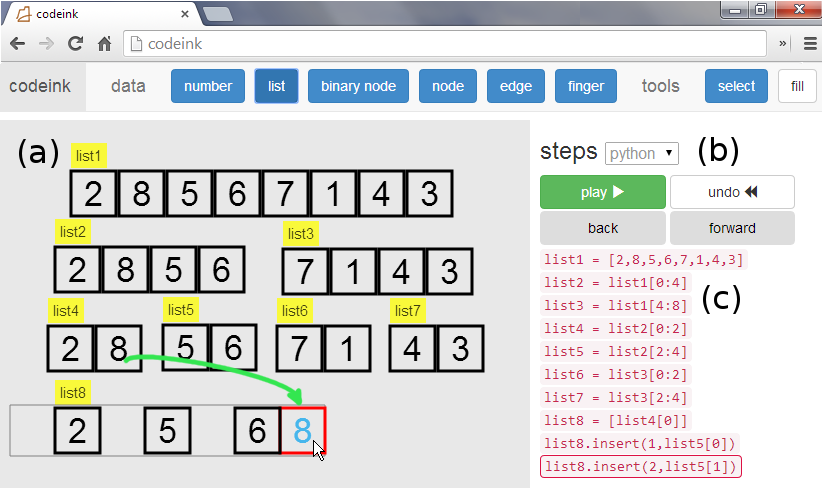
\includegraphics[width=\columnwidth]{img/frontpage-mergesort.png}
\end{center}

\caption{CodeInk enables students and instructors to trace algorithms on
examples by direct manipulation. The user can (a) compose and manipulate
data structures, (b) step through the recorded trace, and (c) see each
step translated into a line of Python code or an English explanation.}

\label{fig:codeink-intro}
\end{figure}


We hypothesize that a much better user interface for teaching and learning
algorithms would (a) afford direct manipulation of data structures, and (b)
record the trace in a structured format that can be disseminated and discussed.

To explore this hypothesis, we built \emph{CodeInk}, a Web-based system for tracing
algorithms by direct manipulation (DM). CodeInk includes a DM gesture set that
enables users to manipulate lists, trees and graphs rather than drawing (and re-drawing)
static snapshots. All manipulationsare recorded as
interactive program steps, in Python or English, providing
three main benefits: feedback on user interactions, navigation through the
trace, and a format that can be easily disseminated and analyzed as a basis for
discussion. 

This paper makes three main contributions:

\begin{comment}
\fig{fig:codeink-intro} shows how an instructor can explain the merge sort
algorithm in CodeInk by dragging an example list onto the canvas, selecting
sublists with a rectangular selection, dragging them away to create copies, then
merging elements by dragging them into a new sorted list
(\fig{fig:codeink-intro}a).
Every interaction is interpreted as a step in Python (\fig{fig:codeink-intro}c).
The trace can then be shared with students, who can navigate through it by
single-stepping or clicking on steps (\fig{fig:codeink-intro}b), and then trace
the algorithm for themselves on a new example. Their own trace can be shared
with instructors as a basis for feedback on not just the final output, but also the
process by which the list was sorted.
\end{comment}


\begin{enumerate}\itemsep0pt

\item A  novel direct manipulation (DM) gesture set for tracing algorithm
behavior on lists, trees and graphs.

\item CodeInk, a system for tracing algorithms that implements the DM
gesture set and records traces as interactive, sharable program steps.

\item An initial evaluation of CodeInk's viability in a controlled
study. Students watched CodeInk-produced traces to learn a new algorithm
and then used CodeInk to trace the algorithm on a new example to
solidify their understanding.

\end{enumerate}

% \pg{talk broader about future implications for this sort of technique}
%%% missed that this was a comment and edited it (RD)
\begin{comment}
While our focus is on enhancing algorithm traces for CS education, we believe the
ability to directly manipulate data structures and record those interactions as
program steps may be more broadly applicable. for the general programmer, it may
enable better visualization and exploration of an algorithm's design. We
conclude this paper with a discussion of future work.
\end{comment}
